\chapter{The Modules}

\section{Introduction}
Figure \ref{normalwin} left panel shows the NuSIM graphical interface. Left clicking on any of the coloured boxes will bring up an options menu for different modes of the module, and left clicking on the module will bring up the options menu for the chosen mode. 

At the bottom of the window there are four grey boxes. The "supervisor" button brings up the main time control of the simulation. The first entry is the total time of the simulation in seconds, and the second entry is the update rate of the diagnostics plots in terms of number of events. It is advisable to set the update rate of the diagnostics window high, since the plotting slows down the simulations speed.

The second grey button "Switch to satellite modules" switches the main window to the satellite control window shown in Figure \ref{normalwin} right panel. This is the control window of the satellite and mainly deals with the loading of databases and setting the space craft pointing. The modules available through this window are described in detail in \ref{ssm}.

The third grey button toggles the displaying of the diagnostics window.

The final button starts the simulation.

\begin{figure}[bt]
  \begin{minipage}[c]{0.48\linewidth}
    \begin{center}
      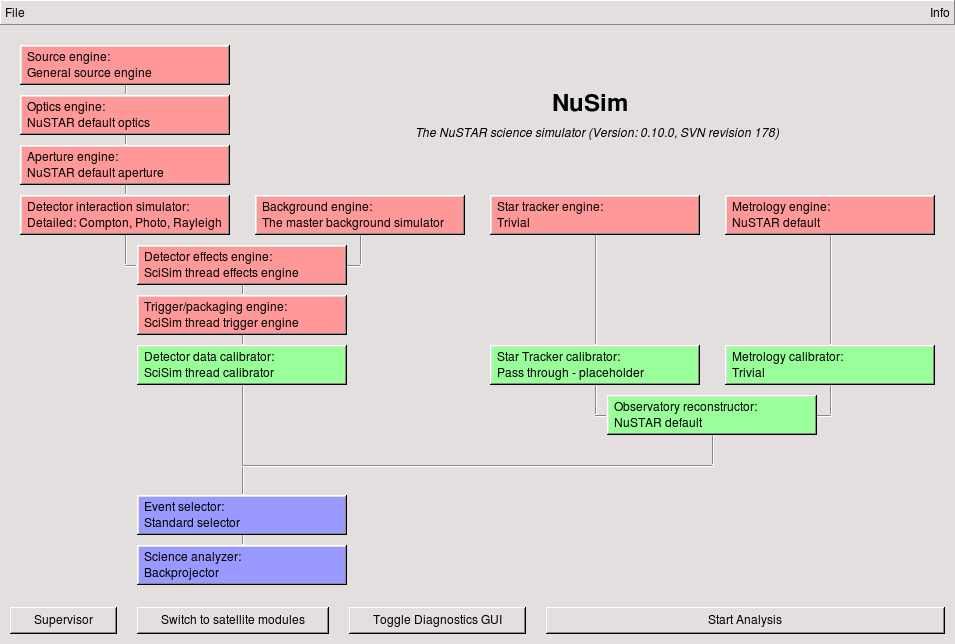
\includegraphics[scale=0.27]{images/MainWindowNormalMode.png}  
    \end{center}
  \end{minipage}
  \hspace{0.04\linewidth}
  \begin{minipage}[c]{0.48\linewidth}
    \begin{center}
      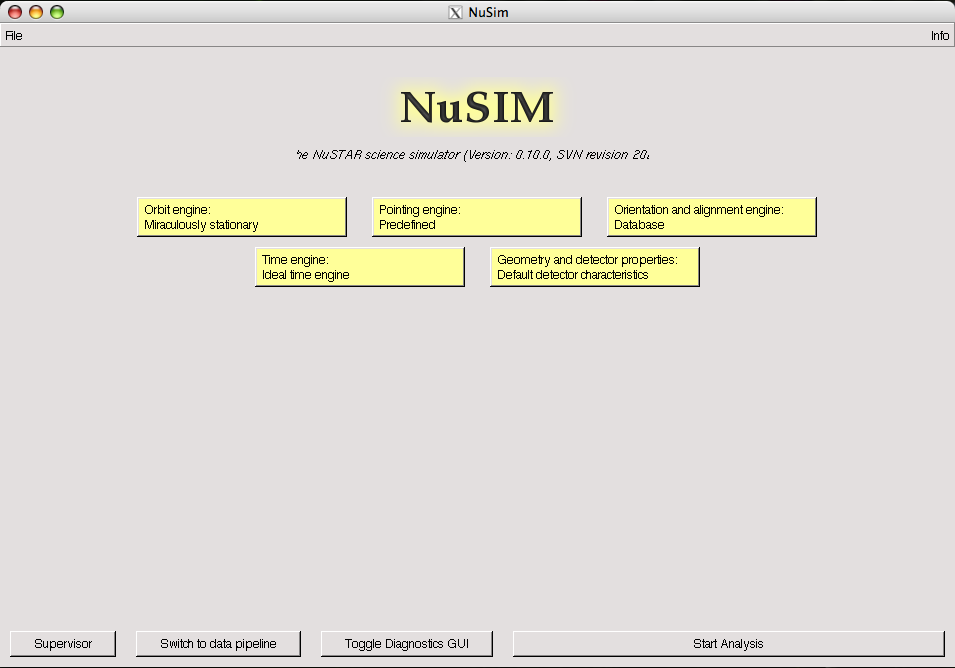
\includegraphics[scale=0.2]{images/satellitegui.png}  
    \end{center}
  \end{minipage}
  \caption{\label{normalwin} Illustration of the main NuSIM GUI window (left) and satellite module window (right).}
\end{figure}

\subsection{Universal Saver and Loader: Saving and loading NuSIM simulations}
There are a variety of output file formats in NuSIM. Each of these will be described under their respective module. However, at almost any point in the simulation the user can choose to save the contents of the EVENT object to an ASCII file. The format of this NuSIM file is in detail described in Chapter \ref{outputformat}. 

Under almost every module there are two common options: "Event Saver: Universal saver" and "Event loader: Universal loader". The save option will save the contents of EVENT at that point in the pipeline. The loader will load a NuSIM file and continue the simulation from that point in the pipeline. These two options are mostly used for debugging and testing of the NuSIM functionality.

\section{Satellite super module}\label{ssm}
The satellite super-module (internally represented by the class NSatellite) provides an interface to all other satellite modules, which are required by various other simulation and analysis modules.
\subsection{Orbit engine}
The orbit engine provides information about the current orbit position of the satellite, e.g. altitude, inclination, position in TBD coordinates.

\subsection{Pointing engine}
\begin{figure}[bt]
\begin{center}
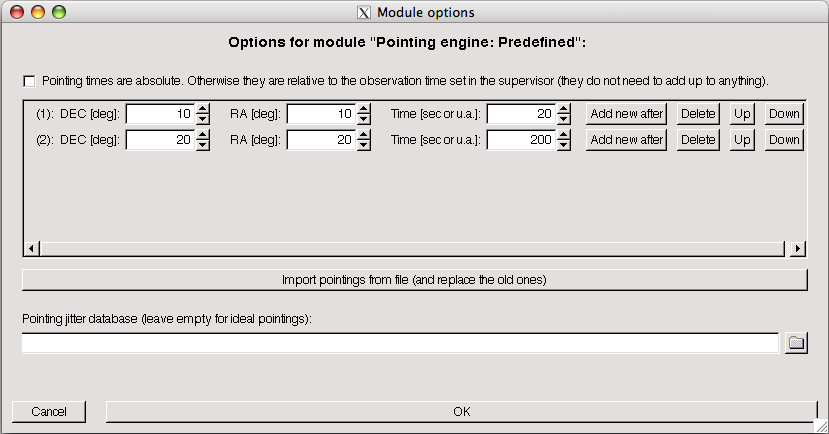
\includegraphics[width=10cm]{images/pointingGUI.png}  
\caption{Pointing module options GUI.}
\label{pointinggui} 
\end{center}
\end{figure}
The pointing engine provides the pointing of the focal plane module in declination and right ascension. Figure \ref{pointinggui} shows the options interface GUI for the pointing module. As illustrated the pointing module allows the user to define multiple pointings. Each pointing requires a coordinate set, a space craft yaw (rotation around z-axis), and an exposure time. Checking the box in the upper left turns the exposure times into absolute seconds, where as leaving it unchecked, the times become relative to the integration time given by the supervisor.

Alternatively the pointings can be loaded in from a file, which will replace any manually entered pointings. Such a pointing file can be for example be created by the source module, which finds an optimal pointing pattern for a given region size.

Finally the last box in the GUI allows the user to load a pointing jitter data base of the spacecraft. 

\subsection{Orientation and alignment engine}
\begin{figure}[tb]
\begin{center}
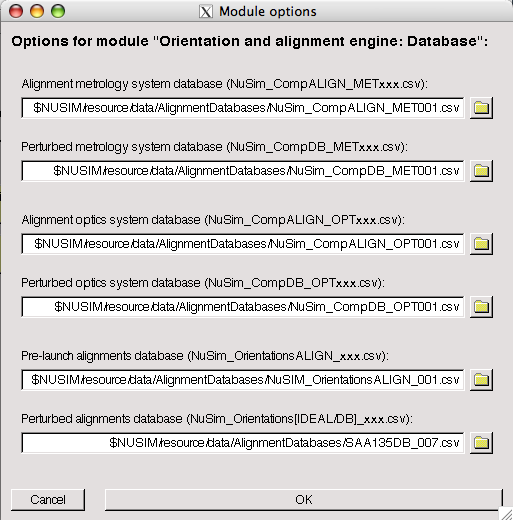
\includegraphics[width=10cm]{images/DBgui.png}  
\caption{Database and alignments options GUI.}
\label{dbgui} 
\end{center}
\end{figure}

The database and alignments module controls input databases and Figure \ref{dbgui} shows the interface options GUI. Each database entry comes in two forms: the ideal alignment of the system as defined "pre-flight", and the "in-flight" alignments which will be subject to thermal perturbations. The databases are divided into 3 groups: the optics, the metrology and star tracker, and finally the rest of the spacecraft alignments. The optics, metrology and star tracker are kept separate so that they can be changed frequently without having to redo the other databases.

\subsection{Time engine}
At the moment the time engine provides the absolute time of the satellite. Modules such as the detector module, the metrology and star tracker module derive their own time from this absolute satellite time and transfer it to the event, star tracker and metrology data sets.   

\subsection{Geometry and detector properties} 

\section{Event pipeline}

\subsection{Source engine}
\begin{figure}[tb]
\begin{center}
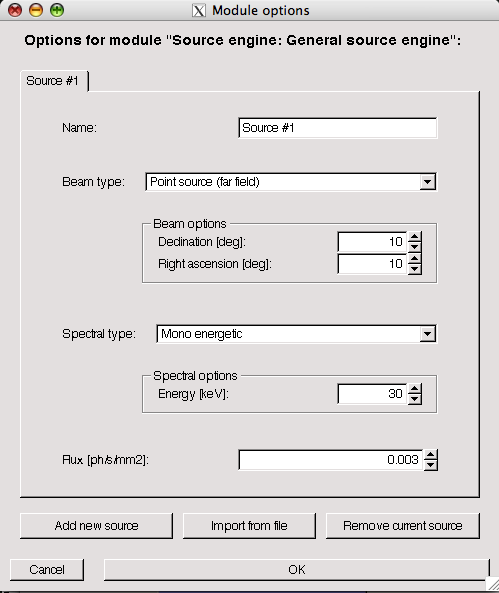
\includegraphics[scale=0.5]{images/sourceGUI.png}  
\caption{Source module options GUI.}
\label{sourcegui} 
\end{center}
\end{figure}
The source module generates the initial spatial and spectral photon distribution for the simulator. Figure \ref{sourcegui} shows the options interface GUI for the source module. Multiple sources can be generated and each source needs to have specified a beam type, spectral type and a flux. It is important to note the the flux here is in (ph/cm$^2$/s). In addition, the flux is always the integrated flux within the given energy bounds set with the spectral options.  

You need to set four parameters for a source: its name, its beam type, its spectral type, and its flux.

The beam type defines the geometry and the position of the source. The position is absolute and in degrees. Make sure that the source and telescope pointing matches. The following beam types are available:
 \begin{itemize}
 \item \textbf{Point source (far field)}: This is a point source at infinity. It requires RA and DEC coordinates in degree.
 \item \textbf{Disk source (far field)}: This creates a disc at infinity defined by its radius. It requires RA and DEC coordinates in degree as well as the radius of the disk in degree.
 \item \textbf{Point source (near field)}: This is used for mimicking a calibration source at a finite distance above the detector. It requires the position of the source (x, y, z in mm).
 \item \textbf{Pencil beam (near field)}: This beam is used to verify CZT detector calibrations. The pencil beam requires a start position as well as a direction (x, y, z in mm), as well as the radius of the beam.  
 \item \textbf{Read from fits file}: This creates a photon field based on a fits intensity image.
 \item \textbf{Normalized combined energy-beam-flux file}: This is the only all-in-one option, a file which contains a normalized (ph/cm$^2$/s/keV/sr) energy-beam-matrix. You do not need to give an additional spectrum or the flux. The file format is described in section \ref{input:3Ddat}.
 \end{itemize}
 
The spectral options are:
\begin{itemize} 
\item \textbf{Mono-energetic}: Requires only the line energy in keV.
\item \textbf{Linear}: Requires the upper and lower boarder of the energy range in keV.
\item \textbf{Power-law}: Requires the upper and lower boarder of the energy range in keV as well as the photon index.
\item \textbf{Broken power-law}: Requires the upper and lower boarder of the energy range in keV, the break energy in keV, as well as the lower and upper photon index.
\item \textbf{Black body}: Requires the upper and lower boarder of the energy range in keV as well as the temperature in keV.
\item \textbf{File with differential flux}: Read differential spectrum from an ASCII file. The spectrum does not require any special normalization besides being 1/keV, since the total flux is as always given by the flux keyword. An example file of the format can be found at:\\
\textbf{\${NUSIM}/resource/data/SourceGenerator.examplespectrum.dat}
\item \textbf{Normalized function in ph/cm$^2$/s/keV}: Requires the upper and lower boarder of the energy range in keV as well as a function in C/C++ form.  You can use all C/C++ function such as exp, log, pow, sqrt, tan, cos, sin, etc. as well as all ROOT functions in the standard ROOT form such as TMath::Gaus(x), etc. Please consult the ROOT manual for all available functions.

Example 1: 7.0e-6*pow(x/10, -1)*exp(-sqrt(x/2.2))

Example 2: TMath::Gaus(x, 67.9, 1.5)

Pay attention to use of "x" for energy and "e" not "E" for the exponent. This is the only spectral option which does not need a flux input, because it is assumed to be correctly normalized.
\end{itemize}

The final required parameter is the flux in $ph/cm^2/s$. This format instead of e.g. $ph/cm^2/s/keV/sr$ had to be chosen to allow to combine each spectrum with each beam. Therefore don't forget to integrate over keV, if you use non-mono-energetic spectra which are given in $keV^{-1}$. This final input is not required for the spectral option "Normalized function in ph/cm2/s/keV" or the beam \"FarFieldNormalizedEnergyBeamFluxFunction\".


For the sources at infinite distance the photons are started randomly from a disk on a sphere surrounding the opening of the optics modules (the module is chosen randomly) to enable the correct simulation of the effective area as a function of incidence angle. The start time is randomly determined (Poisson distribution) according to the source flux. When the start position, start direction and photon energy are determined, the photon is handed over to the optics module for further simulation.


\paragraph{Known issues} 

\begin{itemize}
\item If you have too many sources then no tab is displayed in the GUI. This is a ROOT issue within the TGTab class. If you have too many sources it can on some systems take a long time to display the GUI. This is another ROOT issue within the TGTab class.
\item If you change the beam or spectral type, all parameters get reset
\item Stay away from having sources close to the zenith or nadir (RA, DEC is 0 or 180 degrees) 
\end{itemize}

\vskip 10 true mm

\begin{figure}[tb]
\begin{center}
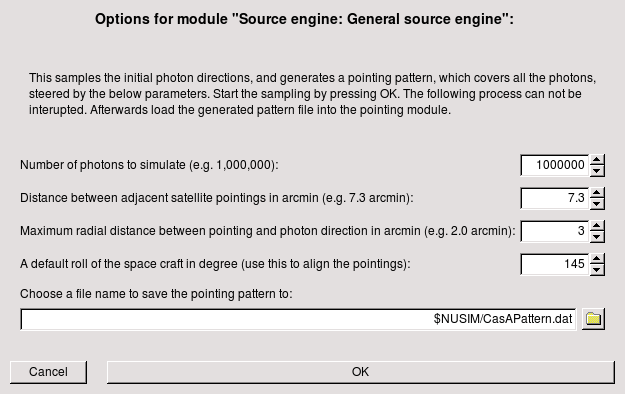
\includegraphics[scale=0.5]{images/pointingpatternGUI.png}  
\caption{GUI for generating pointing patterns.}
\label{pointingpatterngui} 
\end{center}
\end{figure}

A special feature of the source engine is that it can also generate a simple pointing pattern. To do so press the button "Pointing" in the source engine GUI and the GUI see in Fig \ref{pointingpatterngui} should appear. 

The pointing pattern is generated by first simulating a set of photons. The number of photons is given in the first entry box. It should be high enough to sample all sources, but not too high because then the simulation takes too long. 1,000,000 photons seems a reasonable compromise for most situations. For each photon the start direction in RA and DEC is stored. After the simulation, the source region is covered with a rectangular pattern of pointings. The distance between the pointings is given in the second entry field. Since the source field is not necessary rectangular many individual pointings may be not necessary. The last entry in GUI determines how close the pointing direction (i.e. the optical axis of the instrument) must be to a simulated photon in order to accept the pointing. A value of, e.g., 3 arcmin means that one photon must have been simulated within a radius of 3 arcmin of the pointing direction of the instrument. Don't make the value too small, otherwise it's unlikely you have simulated a photon within the disk, and do not make it larger than the half the field-of-view of the instrument.
The next input box gives the yaw (rotation around z-axis) of the space craft, which allows to align the field-of-view (by trial and error at the moment).  
In the bottom entry box you give the name of the file to which the pointings are stored. You have to read this file in the pointing module in order to use it. 

In order to test and verify the coverage of your generated pointing pattern, as well as the evenness of your image, you can make a full simulation with a flat input distribution, e.g. a disk source, which is large enough to cover all pointings.



\subsection{Optics engine}
The optics engine is a full-fledged ray-trace to simulate the actual optics. It incorporates the exact geometry of the optics, and uses externally generated reflectivity files to calculate the reflection of the photons off the mirrors. Additionally it has a module to simulate deflection of the X-ray photons due to mirror imperfections, which will generate the mirror point spread function. The ray-trace also keeps track of single reflections, called "ghost rays", where the photon only reflects off one mirror while passing through.

The module has three options:
\begin{itemize}
\item \textbf{Scattering}: This options turns on the scattering of the photons due to figure errors in the mirrors. Scattering must be on for a science simulation. It is important to note that this is scattering in the reflection sense only, and not of any particle effects.
\item \textbf{Perfect Optics}: This option focuses all rays to one spot. This option should not be used with science simulations and is primarily for debugging.
\item \textbf{Ghost rays}: This option enables the ghost rays. As a default it should be on when running a science simulation. 
\end{itemize}

The input of this module is a photon location, direction and energy handed to it by the source module, and the output is location, direction and energy after the photon has exited the optics.


\subsection{Aperture engine}
The aperture engine places an aperture in the photon path and rejects any photon hitting the aperture. The aperture stop is located 833.187 mm above the detector, and has an opening diameter of 58 mm.

\subsection{Background engine}
\begin{figure}[tb]
\begin{center}
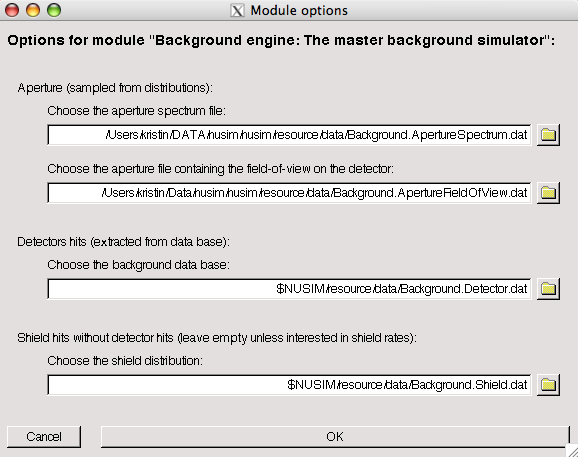
\includegraphics[width=8cm]{images/backgroundgui.png}  
\caption{Background interface options GUI for the "master background simulator".}
\label{bkggui} 
\end{center}
\end{figure}
The background engine draws the background from an external GEANT simulation, combining it with the expected background flux from the sky. This module has three options:
\begin{itemize}
\item \textbf{No Module}. It is possible to run NuSIM without having a background engine.
\item \textbf{Master Background Simulator}. As the name implies this is the actual background option to use when running science simulations. Figure \ref{bkggui} shows the interface options GUI and the files can be found in \textbf{\${NUSIM}/resource/data/}.
\item \textbf{Event Loader: Universal loader}. Allows the user to load a previously saved event list.
\end{itemize}

The master background engine contains 2 different background components, the instrumental background and the aperture background.

The instrumental background has been generated using Geant simulation which comprised the complete expected background: cosmic photons, protons, electron, and positrons, Albedo photons, electrons, positrons, neutrons and protons, trapped protons from passage through the SAA as well as all activation from neutrons and protons. it is split into two parts which have to be set in the GUI: All events which cause interactions in the detector --- this includes detector only and shield and detector interactions --- and shield only interactions.
Although 20.000~hours supercomputer time were available, only 100.000~s of background could be simulated. As consequence all 100~ks the background is reused.
To minimize problems, a random start position in the background file is used and the interaction positions on the detector are modified by randomly switching the detector(s) in which the pattern(s) occurred and by rotating the pattern(s).
The energy, however, is not modified.

The second component is the aperture component, i.e. cosmic diffuse photons which which have an unobscured path to the detector because the aperture is not perfect. However, Beryllium absorption, etc. is taken into account. The input is split into two files, a spectrum and a position pattern on the detectors (which is uneven due to obscuration of the optics). The original input for the data was the Gruber et al. cosmic diffuse spectrum.


\subsection{Detector interactions engine}

The task of the detector interactions engine is to simulate the photons once they enter the detector.
Three simulation modules are available:
\begin{itemize}
 \item \textbf{Only propagate to the detector plane}.
As the name says, this module does not perform simulations inside the detector, but only propagates the photon to the detector plane. This propagation takes into account Beryllium window absorptions.
 \item \textbf{Ideal interactions}.
After propagating the photon to the detector plane as in the previous module, this module performs a simple interaction simulation by only taking into account the interaction depth according to the total absorption probability in CZT along the direction of the original photon. It does not take into account photo effect, fluorescence, Rayleigh or Compton scattering.
 \item \textbf{Detailed: Compton, photo, Rayleigh}.
This is the most frequently used module. It takes account Photo effect including fluorescence photons which can escape the detector (although only the photon with the highest energy is considered), Rayleigh scattering and Compton scattering. Comparisons with Geant4 have shown that the results are within 5\% of Geant4 (version 9.2).
\end{itemize}

\subsection{Detector effects engine}

The main task of the detector effects engine is to convert energies
deposited in the CdZnTe detector by various interactions to charges
measured at each pixel.
There is no time-dependent waveform/sampling information in the output
signal for each pixel.
Inputs are position in detector coordinate system and energy
deposited for each interaction.
The input may be a vector consisting of multiple interactions.
Outputs are total charge at each pixel which has a non-zero charge
deposition.
This engine is followed by the trigger engine which uses the pixel-wise
charge information to determine triggers, veto, which pixels to read
out, etc. This module has 6 options:
\begin{itemize}
 \item \textbf{No module}.
       It is possible to run NuSIM without having a detector effect engine.
 \item \textbf{SciSim}.
       The module converts energy of each interaction to charge only
       in the pixel where interaction occurs with a charge loss database
       derived from observed data.
       The surrounding 8 pixels have zero energy.
       After that, charges in each pixel are integrated.
 \item \textbf{SciSimCIE}.
       The module converts energy to charge
       by a simple multiplicative factor, charge induction efficiency
       (CIE), which depends on interaction position.
       In order to shorten computation time, the CIE values are produced
       by an external software which simulates charge transport and
       induction in the CdZnTe detector based on the Shockley-Ramo theorem.
       These values are filled in a 3-d histogram with a volume of 3-by-3
       pixels in the ROOT file\\
       (\textbf{\${NUSIM}/resource/data/CIE\_450V\_TypicalMuTau.root}).\\
       The ROOT file can be selected via the SciSimCIE GUI in
       Fig~\ref{DEESciSimCIEGUI}.
       At the moment, the detector is assumed to have uniform properties,
       that are temperature ($5{}^\circ\mathrm{C}$),
       electric field (500~V/2~mm), and mobility-lifetime products for
       electrons ($1.0 \times 10^{-2}$~cm$^{2}$ V$^{-1}$)
       and holes ($2.0 \times 10^{-5}$~cm$^{2}$ V$^{-1}$).
       The SciSimCIE module needs to be followed by the SciSim trigger
       engine and the SciSimCIE calibrator.
 \item \textbf{PixSim}.
       (Not yet implemented.)
       The main task of this module is to correctly reproduce grade for
       charge sharing between pixels based on a database measured with
       an X-ray generator. It can not generate accurate spectrum or depth
       plot. Monochromatic peaks are simply Gaussian with zero depth.
       It requires the detector interactions engine as well as incident
       position to the detector.
 \item \textbf{PHE}.
       This module randomly generates event information by reading
       a PHE FITS file.
 \item \textbf{Ideal}.
       This is an ideal detector effects engine with zero energy
       resolution and no charge trapping or diffusion.
\end{itemize}

\begin{figure}[tb]
 \begin{center}
  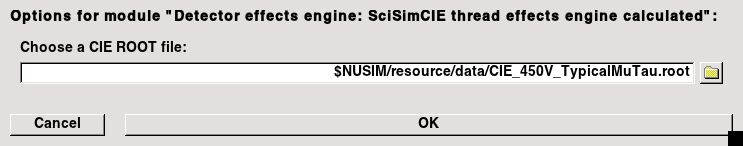
\includegraphics[width=8cm]{images/DetectorEffectEngineSciSimCIEGUI.png}
  \caption{GUI for the SciSimCIE detector effect engine.}
  \label{DEESciSimCIEGUI}
 \end{center}
\end{figure}


\subsection{Trigger engine}

The trigger module represents the trigger and downlink decision hardware
aboard the NuSTAR satellite. It shall decide if an energy deposit in the
shield represents a veto or the pattern on the detector is valid for
a downlink. The following 4 modules are available.
\begin{itemize}
 \item \textbf{No module}.
       NuSIM can run without having a trigger engine.
 \item \textbf{Ideal}.
       This is a simple trigger module which counts the number of
       trigger-activated pixels and generate a shield veto.
 \item \textbf{SciSim}.
       This module is designed to have the same function as the actual
       trigger system and must follow the science detector effects
       engine of SciSim, SciSimCIE, or PixSim.
       Firstly, it searches for a pixel with the highest
       charge and fill event information
       with energies in 3-by-3 pixels which are selected pixel as
       the center and surrounding 8 pixel.
       These 9 energies are used to reconstruct an initial energy
       in the following detector data calibrator for a science
       simulation and energies in the other pixels are ignored.
       Next, the module generates a shield veto flag if an energy
       deposited in the shield is above a lower threshold, which
       can be changed by the interface options GUI for the SciSim
       trigger engine in Fig~\ref{TESciSimGUI}.
       Finally, the module generates a flag to judge whether or not
       this event are in the dead time. This dead-time selection
       can be disabled by the top button in GUI.
 \item \textbf{PHE}.
       This is a specialized trigger engine for the PHE detector
       effects path. At the moment, it does nothing.
\end{itemize}

\begin{figure}[tb]
 \begin{center}
  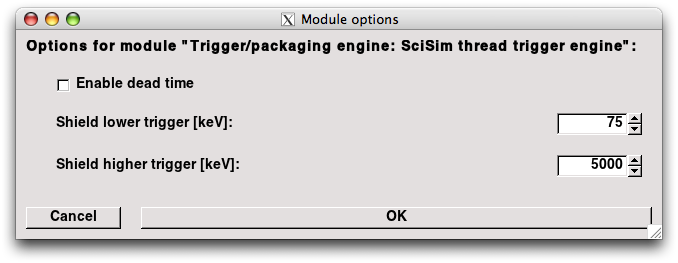
\includegraphics[width=8cm]{images/TriggerEngineSciSimGUI.png}
  \caption{GUI for the SciSim trigger engine.}
  \label{TESciSimGUI}
 \end{center}
\end{figure}

\subsection{Detector data calibrator}

The task of the detector data calibrator is to calibrate the data
produced from a detector effects engine and the following trigger
engine, and generate a level 3 data.
The main calibrations are the depth cut, depth collection, and
the charge share events collection. The following 5 modules are
available.
\begin{itemize}
 \item \textbf{No module}.
       NuSIM can run without having a detector data calibrator.
 \item \textbf{SciSim}.
       This is a detector data calibration engine which belongs to
       the science simulator thread. At this time, There is no
       depth collection or charge share collection.
 \item \textbf{SciSimCIE}.
       This module uses the 9 energies from the SciSim trigger effect
       engine to reconstruct an energy to estimate an incident energy.
       The reconstructed energy is the total energy of triggered pixels
       minus the average energy of the other non-triggered pixels.
       Then, energy scales among events with the different number of
       triggers are calibrated with gain parameters. Although these
       parameters can be changed by the interface options GUI for the
       SciSimCIE calibrator in Fig~\ref{DCSciSimCIEGUI}, the default
       values are already optimized for the current CIE database.
       They may need to be updated if the CIE ROOT file changes.
       In addition, the module sets a flag for depth cut, which is
       an event selection in a depth plot to improve a S/N ratio.
       A boundary curve for depth cut is in a ROOT file,
       \textbf{\${NUSIM}/resource/data/DepthCut.root}.
       The module does not reject bad events, but just set the depth
       cut flag. You can select cleaned events in the following
       event selector module.
 \item \textbf{Ideal}.
       This module is a calibrator which goes with the ideal
       detector effects engine.
 \item \textbf{Replica for background sims}.
       This module is a calibrator for a background simulation.
\end{itemize}

\begin{figure}[tb]
 \begin{center}
  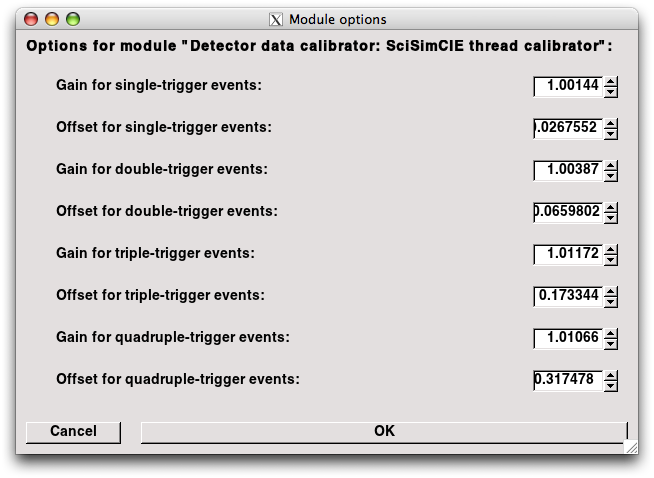
\includegraphics[width=8cm]{images/DetectorCalibratorSciSimCIEGUI.png}
  \caption{GUI for the SciSimCIE detector data calibrator.}
  \label{DCSciSimCIEGUI}
 \end{center}
\end{figure}

\subsection{Event selector}
The Event Selector allows the user to filter the output and produce event-list files. The GUI for this module is shown in Figure \ref{eventgui} The first section gives you options to store the events --- the file name and path are set in the supervisor GUI. Saving as FITS file will produce a simple level 2 fits file that can be loaded into DS9. Saving as ROOT will produce a ROOT file format, and saving as ASCII will prodice the human readable dat file format. In addition, you can create an energy response (incident vs. measured energy) in ROOT file format.

An energy range can be entered to bound the range of the output. If there is no entry then the input range is used.
The top check box allows the user to decide whether they want to save the file before or after the energy filter. The reason is that there is a high energy background which otherwise would be excluded.
The bottom two check boxes enable the users to decide whether they want to filter out events with depth information.

\begin{figure}[tb]
\begin{center}
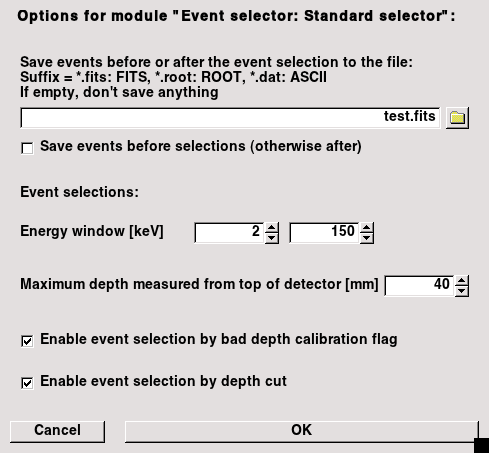
\includegraphics[width=8cm]{images/eventselectorGUI.png}  
\caption{Event selector interface options GUI.}
\label{eventgui} 
\end{center}
\end{figure}

\subsection{Science analyzer}

\section{Metrology and Star tracker pipeline}
\subsection{Metrology engine and calibrator}
The purpose of the metrology engine is to generate data at a rate equivalent to the onboard metrology system. The engine takes the known perturbed aspect of the instrument system and finds the intersection of the metrology laser with the metrology detector. It will then apply noise to the data set simulating the centroiding error of the metrology detector. This is done by applying a Gaussian error to each of the measurement axis. The blurring can be toggled in the metrology GUI, but should be on by default. The 1-sigma error is reported in the database file:\\ \textbf{resource/AlignmentDatabases/NuSim\_CompDB\_MET001.csv} . 

The metrology PSD suffers from non-linearity. In the aspect reconstruction this non-linearity is corrected out, but for testing reasons it can be overridden such that the aspect reconstruction runs without correcting for the non-linearity. The shifts can be toggled in the metrology GUI.

The engine passes the coordinates on to the Observatory Reconstructor for use in deriving the aspect reconstruction.

\subsection{Star tracker engine and calibrator}
Based on the input pointing defined by the pointing engine, the task of the Star Tracker Engine is to generate a quaternion, which defines the rotation between the Camera Head Unit, CHU, to the J2000.0 heliocentric inertial equatorial reference frame, also called VSN (Vernal, Summer, North). The origin is the intersection of the CCD plane with the optical axis of the camera. The CHU z-axis points along the boresight, and x/y axis span the CCD plane.
The output of the Star Tracker is a Quaternion that defines the attitude of the CHU w.r.t. the VSN, such that
\begin{equation} 
x_{CHU}=(Q_{CHU->VSN}) * x_{VSN}. 
\end{equation}
Thus if the a unit vector in the star tracker frame is transformed into the VSN frame by 
\begin{equation}
x_{VSN}=(Q_{CHU->VSN} )^T* x_{CHU}, 
\end{equation}
then RA=atan$(y_{VSN}/x_{VSN})$, DEC=asin$(z_{VSN})$. In the module $(Q_{CHU->VSN})^T$ is produced at a rate equivalent to the onboard Star Tracker. The module will add a Gaussian noise to the transformation to mimic solution error of the Star Camera. The 1-sigma error is reported in the database file:\\ \textbf{resource/AlignmentDatabases/NuSim\_CompDB\_MET001.csv} .

 The transformation is passed on to the Observatory Reconstructor, which interpolates the transformation for a specific time and derives the aspect reconstruction.

\subsection{Observatory reconstructor}
The observatory reconstructor is the set of algorithms that solves the attitude and aspect problems of the NuSTAR observatory, given the metrology and star tracker data. The observatory reconstructor does not have access to the satellite module, which would contain the actual attitude and aspect of the observatory. It is responsible for re-calculating that attitude and aspect, given only a certain number of inputs, which are simulated satellite data.
The inputs to the observatory reconstructor are:
\begin{itemize}
\item The calibrated positions, in local coordinates, at which the metrology lasers impinge on their detectors. These are interpolated in time.
\item The calibrated star tracker data, which is a transformation (quaternion) from local star tracker coordinates to inertial (J2000.0) coordinates. These are interpolated in time. 
\item The on-ground alignment data defining the ideal locations of all the instrument components. Specifically, the pointing of the optical axis in optics bench coordinates, the location and pointing direction of the metrology laser in optics bench coordinates, the location and rotation to the metrology detector from focal plane bench coordinates and to the star tracker from optics bench coordinates.
\end{itemize}
The output from the observatory reconstructor is a transformation from focal plane module coordinates to celestial coordinate $R_{fbin}$.
For extensive details on the algorithm solution, see Chapter \ref{quaternion}, and for the performance details Appendix \ref{aspect}.
